% !TEX root = ../thesis-example.tex
%
\chapter{Metodologia}
\label{Metodologia}

La hipotesis fue ....
por esta razon se utilizo 
A  con los parametros g h j debido a ... presentado en el Capitulo \ref{contexto}

\begin{figure}
	\centering
	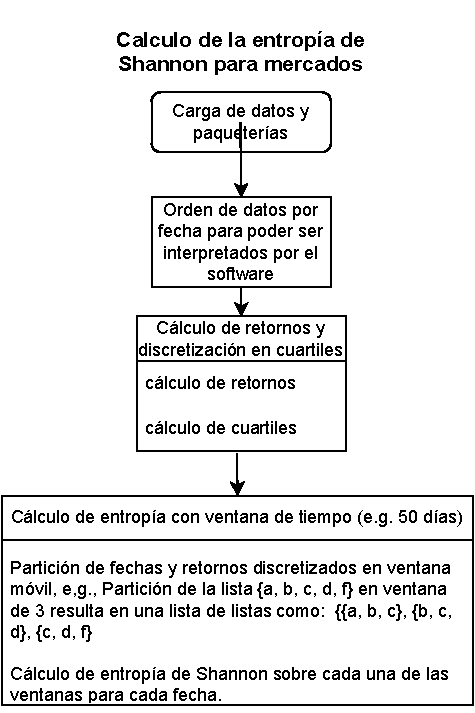
\includegraphics[width=0.7\linewidth]{figures/diagrama_entropia1}
	\caption{}
	\label{diagramaentropia1}
\end{figure}



Pseudo codigo 
\begin{center}
	\begin{tabular}{ |r l| }
		 \hline
		1 & Aplicacion del Metodo de retornos\\
		2 & Calculo de madia moviles utilizando N dias\\ 
		3 & Estimacion gaussiana con sigma igual 3 \\
		 \hline
	\end{tabular}
\end{center}



Apoyo visual 